\documentclass[aps,pra,reprint,superscriptaddress,floatfix]{revtex4-2}

\usepackage{amsmath,amssymb,bm}
\usepackage{braket}
\usepackage{graphicx}
\usepackage{booktabs}
\usepackage{hyperref}

\graphicspath{{figures/}}
\hypersetup{colorlinks=true,citecolor=blue,linkcolor=blue,urlcolor=blue}

\newcommand{\dd}{\mathop{}\!\mathrm{d}}

\begin{document}

\title{Short-pulse sequences as local probes for superconducting-qubit frequency calibration}

\author{Zhouyi Rao}
% Confirm authorship, author order, corresponding email, and ORCID.
\affiliation{Institute of Physics, Chinese Academy of Sciences, Beijing 100190, China}
\affiliation{University of Chinese Academy of Sciences, Beijing 100049, China}

\date{\today}

\begin{abstract}
    \centering
    ABSTRACT PLACEHOLDER: The abstract will be finalized after the main text is confirmed.  It will summarize the motivation, method, and results of the work, and highlight the key contributions and implications for superconducting-qubit frequency calibration.
% Qubit calibration normally extracts frequency information from dedicated
% spectroscopic scans or free evolution between control pulses.  We investigate
% whether a short-pulse sequence can instead contribute directly to calibration
% through the detuning response accumulated during the pulses themselves.  As a
% case study, two orthogonal, zero-delay Ramsey sequences form a local frequency
% discriminator whose first- and third-order response kernels map population to
% detuning.  The cubic correction requires the full three-time kernel rather than
% its time-diagonal restriction.  The short-pulse probe is only locally
% invertible, so its use in a feedback loop additionally requires the drive
% reference to track the predicted qubit frequency and keep each measurement
% inside the calibrated response window.  In a deterministic, seeded
% local-tracking simulation for a 20-MHz target shift, the resulting protocol
% reaches a 5.2-kHz analytically checked residual in six iterations and 984
% counted solver calls, compared
% with an 18.0-kHz residual and 4000 calls for a double-sweep Ramsey baseline.
% These results establish a concrete regime in which short-pulse sequences can
% participate in local calibration, while also identifying response folds and
% reference tracking as the constraints that delimit that role.
\end{abstract}

\maketitle

\section{Introduction}
\label{sec:introduction}

% Superconducting qubits require frequent calibration because transition
% frequencies drift with flux bias, temperature, control conditions, and the
% electromagnetic environment.  Frequency error appears directly as a detuning
% in single-qubit control and propagates into gate, readout, and higher-level
% calibration tasks~\cite{krantz2019quantum,blais2021circuit}.  Modern calibration
% systems therefore organize repeated measurements and parameter updates into
% automated feedback loops~\cite{kelly2018physical,wittler_integrated_2021}.
% Reducing the cost of the elementary frequency measurement is valuable because
% the same primitive is executed across devices and repeated as the processor
% drifts~\cite{rol2017restless,werninghaus_high-speed_2021}.  This motivates a
% broader question: can the short control-pulse sequences already used around a
% working point provide calibration information themselves?

% Ramsey spectroscopy is a robust frequency estimator.  A pair of $\pi/2$
% pulses separated by a variable free-evolution interval converts detuning into
% population oscillations, and the oscillation frequency is extracted from a
% scan.  The scan provides a useful capture range and high precision, but its
% cost scales with the number of delay points and, when two artificial detunings
% are used to determine the sign, with two complete scans.  Fixed-delay Ramsey
% measurements reduce this burden once the frequency is already known locally,
% and have been incorporated into closed-loop stabilization protocols
% ~\cite{vepsalainen2022improving}.  Their local phase response, however, becomes
% ambiguous after phase wrapping.

% Here we test this possibility in a frequency-calibration setting.  We remove
% the free-evolution interval and infer detuning from the response accumulated
% during two finite control pulses.  Orthogonal analysis branches form an odd
% differential signal whose slope is determined by a response kernel.  Such
% control-time response functions connect temporal sensing to driven-qubit
% dynamics~\cite{herb2024quantum,lin2025application}.  They suggest that a short
% pulse can be more than an operation surrounding a calibration experiment: its
% transient response can itself be the probe.  The question is then not only
% whether this response contains frequency information, but whether that local
% information can remain valid as a calibration loop moves the device.

% Two constraints are central.  First, the short-pulse response is nonlinear and
% only locally invertible; its leading correction depends on the full three-time
% response kernel.  Second, if the feedback loop changes the flux bias while the
% drive remains fixed, the qubit can leave the discriminator's monotonic window,
% corrupting both the frequency estimate and the subsequent controller update.

% Our central result is that short-pulse sequences can participate in
% closed-loop frequency calibration when these two constraints are controlled.
% A full three-time response kernel supplies the local cubic inverse.  A secant
% estimate of the frequency--flux slope then predicts the transition frequency
% at the next bias point.  Driving at this predicted frequency keeps the pulse
% response inside its calibrated window, while the feedback residual remains
% defined relative to the fixed target.  The response kernel and drive tracking
% therefore play supporting but distinct roles: one extracts information from
% the short sequence, and the other preserves the validity of that information
% along the calibration trajectory.

% We first derive the short-pulse discriminator and its local inverse.  We then
% separate drive tracking, which preserves measurement validity, from the flux
% update, which closes the control loop.  Numerical tests compare the local
% probe with Ramsey strategies using frequency errors recomputed from the
% analytic simulation model and instrumented solver counts.  This ground-truth
% check is separate from the independent measurement protocol specified for
% \textsc{Verify}. Besides demonstrating a useful operating regime,
% the comparison exposes a negative result: simply placing a short-pulse method
% before Ramsey in a coarse-to-fine workflow can cost more than Ramsey alone.
INTRODUCTION PLACEHOLDER: The introduction will be finalized after the main text is confirmed.  It will motivate the work, summarize the method, and highlight the key contributions and implications for superconducting-qubit frequency calibration.

\newpage

\section{System and calibration task}
\label{sec:system}

\subsection{Flux-tunable transmon and calibration objective}
\label{sec:system-objective}

We consider a flux-tunable transmon qubit~\cite{krantz2019quantum} controlled through a calibrated flux-bias coordinate $\Phi$. 
%Experimentally, $\Phi$ is controlled through a room-temperatue bias voltage $V_{\mathrm b}$ using a separately characterized voltage-to-flux conversion, as detailed in the Supplemental Material.
In the transmon regime, the flux dispersion of the qubit angular transition frequency is approximately given by~\cite{koch2007charge}
%
\begin{equation}
\begin{split}
\hbar\omega_{01}(\Phi)
\simeq{}&
\sqrt{8E_CE_J(\Phi)}-E_C, \\
% E_J(\Phi)
% ={}&
% E_{J,\Sigma}
% \sqrt{
% \cos^2\left(\pi\Phi/\Phi_0\right)
% +
% d^2\sin^2\left(\pi\Phi/\Phi_0\right)
% },
\label{eq:transmon-dispersion}
\end{split}
\end{equation}

Equation~\eqref{eq:transmon-dispersion} describes the flux dependence of the
transition frequency and thus provides the physical basis for frequency
calibration through flux-bias tuning. The calibration objective is to find a
flux bias $\Phi_\star$ such that
%
\begin{equation}
\left|\omega_{01}(\Phi_\star)-\omega_{\mathrm{tar}}\right|
\leq \epsilon_\omega,
\label{eq:calibration-success}
\end{equation}
%
where $\omega_{\mathrm{tar}}$ is the target angular transition frequency and
$\epsilon_\omega$ is the prescribed tolerance. This condition defines calibration success; the subsequent workflow monitors
the verified working point and initiates independent verification or
recalibration when drift is suspected.

In practice, a previously characterized frequency--flux map may no longer be
accurate at the target tolerance because of slow shifts in the effective flux
offset or device parameters\cite{paladino2014noise,vepsalainen2022improving}. We therefore formulate the calibration without
assuming an up-to-date quantitative map $\omega_{01}(\Phi)$: the controller
operates in the calibrated flux coordinate and obtains the local frequency
information required for bias updates directly from measurements.

Figure~\ref{fig:system-protocol}(a) summarizes this calibration setting. The
full dispersion illustrates the physical tunability of the qubit, while the
inset shows a local trajectory from the seed bias toward the target frequency.
% The displayed dispersion is withheld from the controller, which uses only the
% frequency information obtained at the visited bias points.

\begin{figure*}[t]
    \centering
    
\includegraphics[width=0.9\textwidth]{figures/fig1/fig1-system-protocol.pdf}
    \caption{Schematic overview of the physical system, measurement probes,
    and calibration protocol. (a) Qubit frequency dispersion, with an inset showing the seed bias, target
    frequency, and successive points of the local calibration trajectory. The
    complete dispersion is withheld from the calibration controller. (b) Timing diagrams for scanned Ramsey,
    fixed-delay Ramsey, and the bipartite short-pulse probe. (c) The
    \textsc{Acquire--Track--Verify--Lock} protocol, with
    \textsc{Reacquire} recovery and a terminal safe hold. Only
    \textsc{Track} changes the flux bias; \textsc{Verify} freezes the
    candidate bias for independent confirmation, and \textsc{Lock} performs
    long-term monitoring. Solid, dashed, and dotted arrows denote forward,
    fallback, and failure transitions, respectively.}
    \label{fig:system-protocol}
\end{figure*}

% A calibration cycle combines three distinct operations: measurement, estimation, and tuning. A measurement executes a probe at fixed $\Phi_n$ and returns population data. An estimator maps these data to $\widehat{\Delta}_n$ and $\widehat{\omega}_{01,n}$, and a tuning step changes the flux bias. Repeated cycles locate the target working point. Stabilization, in contrast, suppresses subsequent drift around an established working point and is not the primary task considered here.

\subsection{Ramsey and bipartite short-pulse probes}
\label{sec:system-probes}

At each calibration iteration, the qubit is interrogated at a fixed flux bias
by a control sequence followed by population readout. We refer to this
pulse-and-readout operation as a measurement probe. We consider two types of
probes: Ramsey probes and bipartite short-pulse probes. The driven dynamics of
both probes are described by an effective two-level Hamiltonian. In a frame
rotating at the drive frequency $\omega_d$ and under the rotating-wave
approximation~\cite{krantz2019quantum,blais2021circuit},
\begin{equation}
\begin{aligned}
\frac{H(t,\Phi)}{\hbar}
={}&
\frac{\Delta(\Phi)}{2}\sigma_z
+
\frac{\Omega(t)}{2}
\left[
\cos\varphi(t)\sigma_x
+
\sin\varphi(t)\sigma_y
\right],
\\
\Delta(\Phi)
={}&
\omega_{01}(\Phi)-\omega_d .
\end{aligned}
\label{eq:hamiltonian}
\end{equation}
%
Here $\Delta(\Phi)$ is the angular-frequency detuning, while $\Omega(t)$ and
$\varphi(t)$ are the drive envelope and phase. The detuning term connects the
unknown transition frequency to the driven dynamics. Ramsey and short-pulse
probes use the distinct control sequences shown in
Fig.~\ref{fig:system-protocol}(b) to infer this detuning from population
readout. once $\widehat\Delta$ is obtained, the transition frequency follows
as $\widehat\omega_{01}=\omega_d+\widehat\Delta$.

% Figure~\ref{fig:system-protocol}(b) compares the timing structures of the
% two probe types. We first consider the Ramsey probe, which uses two nominal
% $\pi/2$ pulses separated by a free-evolution interval
% $\tau$~\cite{ramsey1950molecular}.

We first consider the Ramsey probe, which uses two nominal $\pi/2$ pulses
separated by a free-evolution interval $\tau$~\cite{ramsey1950molecular}. For an ideal Ramsey sequence with analysis phase $\varphi$ and Ramsey-fringe visibility $C$, the measured population can be written as
\begin{equation}
    p_R(\Delta; \tau, \varphi) = \frac{1}{2}\left[ 1 + C\cos(\Delta\tau + \varphi) \right],
    \label{eq:ramsey-response}
\end{equation}
We use scanned Ramsey, which samples
multiple values of $\tau$, for wide-range frequency estimation. As a local
baseline, we instead fix $\tau=\tau_0$ and use two orthogonal analysis phases
to recover the detuning from measured quadratures within the unambiguous phase
range~\cite{vepsalainen2022improving}. 
% The data processing and choice of
% $\tau_0$ are specified in Appendix~\ref{app:methods}.

We next turn to the bipartite short-pulse probe. Unlike the Ramsey probe,
it contains no separate free-evolution interval and instead applies a common
preparation rotation of angle $\alpha$ immediately
followed by one of two analysis rotations whose phases differ by $\pi$~\cite{herb2024quantum}:
\begin{equation}
    R_y(\alpha) \longrightarrow R_{+x}(\alpha) \quad\text{or}\quad R_y(\alpha) \longrightarrow R_{-x}(\alpha).
    \label{eq:bipartite-sequences}
\end{equation}

Here $\alpha = \int \Omega(t) \dd t$ is determined from the pulse envelope and duration. Varying $\alpha$ changes the differential detuning response and therefore the response coefficients and validated operating range introduced in Sec.~III.

We refer to these two sequences as the $+X$ and $-X$ branches and denote
their final excited-state populations by $p_{+X}$ and $p_{-X}$,
respectively. We define the corresponding differential observable as
\begin{equation}
    p_{\mathrm d}
    =
    \frac{p_{+X}-p_{-X}}{2}.
    \label{eq:pdiff}
\end{equation}

Detuning acts during the finite control pulses and changes the measured branch
populations. Their difference provides a first-order-sensitive local frequency
observable when
\begin{equation}
    \left.
    \frac{\partial p_{\mathrm d}}{\partial\Delta}
    \right|_{\Delta=0}
    \neq 0.
    \label{eq:local-identifiability}
\end{equation}
This condition is necessary for local inversion but does not guarantee an
unambiguous response over an unrestricted detuning range. Section~III
quantifies the local response and establishes its validated operating interval.


\subsection{Calibration workflow}
%  and independent validation}
\label{sec:calibration-workflow}

The local-identifiability condition applies at a fixed bias, whereas a bias
update can move the qubit outside the validated short-pulse range. We therefore
embed the local probe in the
\textsc{Acquire--Track--Verify--Lock} workflow shown in
Fig.~\ref{fig:system-protocol}(c), supplemented by
\textsc{Reacquire} and terminal \textsc{SafeStop} states. This architecture is
motivated by automated qubit calibration and closed-loop frequency
feedback~\cite{kelly2018physical,wittler_integrated_2021,
vepsalainen2022improving}.

At iteration $n$, the measurement detuning and target residual are
%
\begin{equation}
\Delta_n=\omega_{01}(\Phi_n)-\omega_{d,n},
\qquad
r_n=\omega_{01}(\Phi_n)-\omega_{\mathrm{tar}}.
\label{eq:detuning-and-residual}
\end{equation}
%
The detuning $\Delta_n$ determines whether the local probe remains valid,
whereas $r_n$ determines whether the target has been reached. A flux-bias
update changes the physical working point to reduce $r_n$; a drive-reference
update controls the detuning of the next measurement without changing the
target.

For both \textsc{Acquire} and \textsc{Track}, an estimate becomes a target
candidate when
%
\begin{equation}
|\widehat r_{x,k}|
+z_{1-\beta}\sigma_{x,k}
\leq\epsilon_{\mathrm{enter}},
\qquad
x\in\{\mathrm{acq},\mathrm{tra}\},
\label{eq:target-entry-condition}
\end{equation}
%
where $\sigma_{x,k}$ is the uncertainty of the estimated target residual and
$z_{1-\beta}$ is the prescribed confidence multiplier.

In \textsc{Acquire}, scanned Ramsey estimates the current qubit frequency and
initializes the drive. An estimate satisfying
Eq.~\eqref{eq:target-entry-condition} is routed directly to
\textsc{Verify}; otherwise, it seeds \textsc{Track}. Only \textsc{Track}
updates the flux bias, using the short-pulse frequency estimate while updating
the drive reference to keep subsequent measurements within the validated
range. When a \textsc{Track} estimate satisfies
Eq.~\eqref{eq:target-entry-condition}, the bias is frozen and passed to
\textsc{Verify}. A failed local-validity check instead enters
\textsc{Reacquire}.

\textsc{Verify} uses independent Ramsey measurements at the frozen bias.
Calibration is confirmed only after $N_{\mathrm{verify}}$ consecutive
measurements satisfy
%
\begin{equation}
|\widehat r_{\mathrm{ver},j}|
+z_{1-\beta}\sigma_{\mathrm{ver},j}
\leq\epsilon_{\mathrm{final}}.
\label{eq:verification-condition}
\end{equation}
%
A correctable verification error returns to \textsc{Track}, whereas a lost
frequency reference or an error outside the local recovery range enters
\textsc{Reacquire}.

After successful verification, \textsc{Lock} holds the verified bias and uses
periodic low-cost short-pulse measurements to monitor drift. Detected drift or
a scheduled audit returns the protocol to \textsc{Verify}. Before a monitor
residual is used for routing, its applied bias and drive are checked and its
probe detuning must satisfy the same local-validity condition in
Eq.~\eqref{eq:track-range-condition}. A large frequency jump, a failed
monitor-validity check, or loss of the local reference enters
\textsc{Reacquire}.
\textsc{Reacquire} repeats the wide-range acquisition and applies the same
routing rule as \textsc{Acquire}. Cancellation, budget exhaustion, or a safety
interlock enters \textsc{SafeStop}. Detailed thresholds and schedules are
specified in Appendix~\ref{app:methods}.
% The local-identifiability condition above concerns a fixed bias, whereas a
% calibration update can move the qubit beyond the invertible short-pulse range.
% We therefore use the \textsc{Acquire--Track--Verify--Lock} workflow in
% Fig.~\ref{fig:system-protocol}(c), with \textsc{Reacquire} recovery and a
% terminal \textsc{SafeStop}. \textsc{Acquire} establishes a wide-range absolute
% reference; \textsc{Track} alone performs calibration bias updates;
% \textsc{Verify} independently confirms a frozen candidate; and \textsc{Lock}
% monitors without correcting. \textsc{Reacquire} restores a lost reference,
% whereas \textsc{SafeStop} applies a safe bias hold. This separation follows
% the general setting of automated qubit calibration and closed-loop frequency
% feedback~\cite{kelly2018physical,wittler_integrated_2021,
% vepsalainen2022improving}.

% A probe returns population data, an estimator converts them into a frequency
% estimate and uncertainty, and the controller may update the physical bias. A
% separate drive-reference update changes only the reference of the next
% measurement. These operations are governed by
% %
% \begin{equation}
% \Delta_n
% =
% \omega_{01}(\Phi_n)-\omega_{d,n},
% \qquad
% r_n
% =
% \omega_{01}(\Phi_n)-\omega_{\mathrm{tar}}.
% \label{eq:detuning-and-residual}
% \end{equation}
% %
% The measurement detuning $\Delta_n$ guards local-probe validity, whereas the
% residual $r_n$ tests the fixed target. A bias update reduces $r_n$ by moving
% the working point; a drive update controls $\Delta_n$ without reducing
% $r_n$ or redefining the target.

% With $z_{1-\beta}$ denoting the prescribed confidence multiplier, define
% %
% \begin{align}
% U_{x,k}&=|\widehat r_{x,k}|+z_{1-\beta}\sigma_{x,k},
% &x&\in\{\mathrm{acq},\mathrm{tra},\mathrm{ver},\mathrm{loc}\},
% \label{eq:track-verify-statistics}\\
% \epsilon_{\mathrm{hold}}&<\epsilon_{\mathrm{final}}
% <\epsilon_{\mathrm{enter}}<\Delta_{\mathrm{val}}.
% \label{eq:threshold-hierarchy}
% \end{align}
% %
% Here $U_{x,k}$ is always a target-residual statistic. In contrast,
% $\Delta_{\mathrm{val}}$ bounds the probe detuning in
% Eq.~\eqref{eq:track-range-condition}; it must not be applied directly to
% $|\widehat r_{\mathrm{tra},k}|$. The ordering in
% Eq.~\eqref{eq:threshold-hierarchy} compares policy scales, not interchangeable
% observables.

% \textsc{Acquire} routes a reliable off-target estimate to \textsc{Track}. An
% acquired estimate or an accepted \textsc{Track} estimate instead becomes a
% target candidate when
% %
% \begin{equation}
% U_{x,k}\leq\epsilon_{\mathrm{enter}},
% \label{eq:target-entry-condition}
% \end{equation}
% %
% for $x\in\{\mathrm{acq},\mathrm{tra}\}$. The bias is then frozen and the
% protocol enters \textsc{Verify}; neither state can declare success. A valid
% off-target \textsc{Track} estimate instead produces the bounded update of
% Sec.~\ref{sec:calibration-protocol} and remains in \textsc{Track}. A failed
% range, branch-continuity, or sensitivity check enters \textsc{Reacquire}
% rather than extrapolating the local inverse.

% \textsc{Verify} uses measurements independent of the short-pulse estimator
% and its convergence history. Calibration is confirmed only after
% $N_{\mathrm{verify}}$ consecutive measurements at the frozen bias satisfy
% %
% \begin{equation}
% U_{\mathrm{ver},j}\leq\epsilon_{\mathrm{final}}.
% \label{eq:verification-condition}
% \end{equation}
% %
% A reliable verification miss returns to \textsc{Track}; an ambiguous or
% locally invalid verification result enters \textsc{Reacquire}. Measurements
% collected in \textsc{Track} never count toward $N_{\mathrm{verify}}$, even
% when they satisfy Eq.~\eqref{eq:target-entry-condition}.

% Successful verification enters \textsc{Lock}, which retains the verified bias
% and seeks $U_{\mathrm{loc}}\leq\epsilon_{\mathrm{hold}}$. A clear monitor
% result remains in \textsc{Lock}; repeated suspicion or a scheduled Ramsey
% audit enters \textsc{Verify}, while a large jump or lost reference enters
% \textsc{Reacquire}. The latter repeats wide-range acquisition and routes its
% seed by the same rule as \textsc{Acquire}. Budget exhaustion, cancellation,
% or an interlock instead enters terminal \textsc{SafeStop}.

% Response calibration, held-out response validation, closed-loop verification,
% and long-term monitoring use distinct data roles. Their thresholds, budgets,
% and schedules are given in Appendix~\ref{app:methods}. 
% % The present study
% % reports deterministic solver cost and analytic residuals, not hardware
% % $T_{\mathrm{hit}}$ or long-term locking data.

% Section~\ref{sec:inference-calibration} constructs only the estimator and the
% bias- and drive-reference updates used within \textsc{Track}; all state
% transitions and the definition of calibration success remain those above.

\section{Short-pulse frequency inference and calibration}
\label{sec:inference-calibration}

We now specify the local \textsc{Track} branch introduced in Sec.~II.C.
A usable tracking iteration must convert the differential population into a
frequency estimate, move the physical working point toward
$\omega_{\mathrm{tar}}$, and keep the next measurement within the validated
response interval as the qubit frequency changes. We therefore derive the
short-pulse differential response, construct its nonlinear local inverse
together with an explicit validity boundary, use the resulting frequency
estimate in a bounded flux-bias update, and update the drive reference to
preserve the local measurement condition. Together, these elements specify how, and within what limits, short-pulse
frequency information can be incorporated into closed-loop flux-bias
calibration.


\subsection{Short-pulse differential response}
\label{sec:differential-response}

To characterize how detuning is encoded in
Eq.~\eqref{eq:pdiff}, we regard the differential population as a
functional of a time-dependent detuning $\Delta(t)$. Following the general
framework of linear and nonlinear response
theory~\cite{kubo1957statistical,mukamel1995principles}, we expand the
differential population around the resonant control evolution as
%
\begin{equation}
\begin{aligned}
p_{\mathrm d}[\Delta]
={}&
p_{\mathrm d}^{(0)}
+
\sum_{m=1}^{\infty}
\frac{1}{m!}
\int_0^T\!\dd t_1\cdots\int_0^T\!\dd t_m
\\
&\quad\times
k_m(t_1,\ldots,t_m)
\prod_{j=1}^{m}\Delta(t_j).
\end{aligned}
\label{eq:differential-volterra}
\end{equation}
%
Here $k_m(t_1,\ldots,t_m)$ is the symmetrized $m$th-order
detuning-response kernel of the complete bipartite short-pulse probe. It
quantifies the joint contribution of detuning at the times
$t_1,\ldots,t_m$ to the final differential population, and $T$ is the total
sequence duration. The response-function derivation, including time ordering
and nested commutators, is given in the Supplemental Material.

For scalar local frequency estimation, we restrict attention to the
quasi-static regime in which detuning variations during a single short
sequence are negligible, so that $\Delta(t)\simeq\Delta$. This approximation
does not preclude drift between repetitions or feedback iterations.

For the ideal $+X/-X$ probe defined in
Eq.~\eqref{eq:bipartite-sequences}, detuning reversal interchanges the branch
responses,
$p_{+X}(-\Delta)=p_{-X}(\Delta)$. The differential combination therefore
satisfies $p_{\mathrm d}(-\Delta)=-p_{\mathrm d}(\Delta)$. In particular,
$p_{\mathrm d}^{(0)}=0$, and all even-order terms in
Eq.~\eqref{eq:differential-volterra} vanish. The local response can thus be
written as
%
\begin{equation}
p_{\mathrm d}(\Delta)
=
G_1\Delta
+
\frac{G_3}{3!}\Delta^3
+
\mathcal O(\Delta^5),
\label{eq:short-pulse-cubic-response}
\end{equation}
%
where $G_1$ and $G_3$ are the first and third derivatives of
$p_{\mathrm d}$ with respect to $\Delta$ at resonance. The coefficient
$G_1$ determines the local sensitivity, while $G_3$ gives the leading
nonlinear correction.

For the experimental implementation, we separate the response measurements
into calibration and validation data. From the response-calibration data, we
obtain $G_1$ and $G_3$ through an offline, measurement-based kernel
calibration. Calibrated Virtual-$Z$ phase insertions are applied at selected
times within the two control branches, and finite differences of the
resulting branch populations sample the detuning-response derivatives. In
the quasi-static limit, the integrated coefficients are
%
\begin{equation}
\begin{aligned}
G_1
&=
\int_0^T k_1(t)\,\dd t,
\\
G_3
&=
\iiint_{[0,T]^3}
k_3(t_1,t_2,t_3)\,
\dd t_1\dd t_2\dd t_3 .
\end{aligned}
\label{eq:g1-g3}
\end{equation}
%
The Virtual-$Z$ operations follow
Ref.~\cite{mckay2017efficient}. The finite-difference construction and
three-time sampling scheme used to obtain the response kernels are detailed
in the Supplemental Material.

Experimental imperfections may nevertheless produce a nonzero measured
differential signal at resonance. We therefore define
%
\begin{equation}
\widetilde p_{\mathrm d}
=
p_{\mathrm d}^{\mathrm{meas}}-b_0,
\label{eq:corrected-differential-response}
\end{equation}
%
where $b_0$ is the zero-detuning intercept estimated from the
response-calibration data and held fixed thereafter. This operation corrects
a differential-population offset; it does not shift the frequency reference.

For comparison, an odd-polynomial fit to the corrected quasi-static response
provides a separate check of the integrated coefficients but is not used to
generate the coefficients supplied to the main feedback protocol. Once
$G_1$, $G_3$, and $b_0$ have been fixed, separately acquired
response-validation data are used to establish
$\Delta_{\mathrm{val}}$ and to assess residual symmetry breaking through
$p_{\mathrm{even}}(\Delta)
=[\widetilde p_{\mathrm d}(\Delta)
+\widetilde p_{\mathrm d}(-\Delta)]/2$.
The even component is treated as a diagnostic of model mismatch rather than
absorbed into the ideal odd response model. This response validation is
distinct from the independent frequency verification used to confirm
calibration success in Sec.~II.C.

The acquisition and partitioning of the calibration and validation data,
together with the sampling schedule, coefficient-reuse range, recalibration
conditions, and associated cost accounting, are specified in
Appendix~\ref{app:methods}.

\subsection{Local frequency estimator}
\label{sec:local-estimator}

The first-order frequency estimate follows from the local slope:
%
\begin{equation}
\widehat\Delta^{(1)}
=
\frac{\widetilde p_{\mathrm d}}{G_1},
\qquad
\widehat\omega_{01}^{(1)}
=
\omega_d+\widehat\Delta^{(1)}.
\label{eq:linear-frequency-estimator}
\end{equation}
%
Its truncation bias increases as the probe moves away from resonance. This
estimate provides the initial value for the cubic inversion and the
first-order reference used to quantify nonlinear-estimation bias in
Sec.~IV.

The main local estimator retains the third-order response and solves
%
\begin{equation}
G_1\widehat\Delta^{(3)}
+
\frac{G_3}{6}
\left(\widehat\Delta^{(3)}\right)^3
=
\widetilde p_{\mathrm d},
\label{eq:cubic-frequency-estimator}
\end{equation}
%
with
$\widehat\omega_{01}^{(3)}
=\omega_d+\widehat\Delta^{(3)}$.
Newton iteration is initialized with $\widehat\Delta^{(1)}$, and the
candidate solution is selected from the branch connected continuously to
$\Delta=0$.

When $G_1G_3<0$, the cubic response has stationary points at
%
\begin{equation}
\left|\Delta_{\mathrm{fold}}\right|
=
\sqrt{-\frac{2G_1}{G_3}}.
\label{eq:response-fold}
\end{equation}
%
Beyond these points, the cubic response is no longer one-to-one, and the same
differential population can correspond to multiple detunings. The response
fold is therefore a mathematical boundary of the truncated cubic model, not
an experimentally established operating range.

We define the validated local operating interval by
%
\begin{equation}
|\Delta|
\leq
\Delta_{\mathrm{val}},
\qquad
\Delta_{\mathrm{val}}
<
|\Delta_{\mathrm{fold}}|
\quad
(G_1G_3<0).
\label{eq:validated-interval}
\end{equation}
%
The value of $\Delta_{\mathrm{val}}$ is established from the held-out
response-validation data using predefined estimator-error and confidence
criteria. It remains necessary when the cubic model has no real fold because
model truncation, measurement noise, and experimental imperfections can
restrict the usable response before a mathematical turnover occurs. Failure
of numerical convergence, branch continuity, or the validated-range check
rejects the estimate and triggers \textsc{Reacquire} rather than extrapolation
of the local inverse.

\subsection{Track initialization and flux-bias update}
\label{sec:calibration-protocol}

Section~II.C defined the state transitions of the complete calibration
workflow. Here we construct the local controller that operates after an
\textsc{Acquire} or \textsc{Reacquire} measurement has supplied the seed
%
\begin{equation}
\left(
\Phi_{\mathrm{seed}},
\widehat\omega_{01,\mathrm{seed}},
\sigma_{\omega,\mathrm{seed}}
\right).
\label{eq:acquired-seed}
\end{equation}
%
The acquired frequency estimate is reused rather than repeated with the
short-pulse probe at the same bias. It initializes the local drive reference
as
$\omega_{d,\mathrm{seed}}
=\widehat\omega_{01,\mathrm{seed}}$ and gives the seed residual
%
\begin{equation}
\widehat r_{\mathrm{seed}}
=
\widehat\omega_{01,\mathrm{seed}}
-
\omega_{\mathrm{tar}}.
\label{eq:seed-residual}
\end{equation}
%
If Eq.~\eqref{eq:target-entry-condition} is already satisfied, the workflow
proceeds directly to \textsc{Lock}. Otherwise, the seed is used to initialize
the local flux-bias update.

Because one bias--frequency pair does not determine a secant sensitivity, the
controller proposes a bounded one-sided step,
%
\begin{equation}
\Phi_1^{\mathrm{prop}}
=
\Phi_{\mathrm{seed}}
-
\chi_\Phi
\operatorname{sgn}(\widehat r_{\mathrm{seed}})
\delta\Phi_{\mathrm{blind}},
\label{eq:blind-step}
\end{equation}
%
where
$\chi_\Phi
=\operatorname{sgn}(\partial\omega_{01}/\partial\Phi)
\in\{-1,+1\}$
specifies the known local monotonic direction. The applied bias $\Phi_1$ is
restricted to the allowed interval $[\Phi_{\min},\Phi_{\max}]$.

Let $\Delta_{\mathrm{blind}}^{\max}$ denote an experimentally established
upper bound on the frequency displacement produced by the applied blind
step. The proposed initialization is admitted to \textsc{Track} only if
%
\begin{equation}
z_{1-\beta}\sigma_{\Delta,\mathrm{seed}}
+
\Delta_{\mathrm{blind}}^{\max}
\leq
\Delta_{\mathrm{val}},
\label{eq:track-entry-condition}
\end{equation}
%
where $\sigma_{\Delta,\mathrm{seed}}$ includes the uncertainty of the acquired
frequency and the implemented seed reference. This condition reserves enough
detuning margin for the first short-pulse measurement after the blind step.
The determination of $\Delta_{\mathrm{blind}}^{\max}$ and the choice of
$\delta\Phi_{\mathrm{blind}}$ are described in
Appendix~\ref{app:methods}.

No measured sensitivity is available before this step, so the first
short-pulse probe at $\Phi_1$ uses
$\omega_{d,1}=\widehat\omega_{01,\mathrm{seed}}$. Its output supplies the
second frequency estimate $\widehat\omega_{01,1}$ and hence the initial
secant sensitivity
%
\begin{equation}
\widehat S_{\Phi,1}
=
\frac{
\widehat\omega_{01,1}
-
\widehat\omega_{01,\mathrm{seed}}
}{
\Phi_1-\Phi_{\mathrm{seed}}
}.
\label{eq:initial-secant-sensitivity}
\end{equation}
%
This initial slope combines the scanned-Ramsey seed with the short-pulse
estimate at $\Phi_1$. The uncertainty assigned to
$\widehat S_{\Phi,1}$ includes the uncertainties of both frequency estimates.

For subsequent iterations, the local sensitivity is estimated from the two
most recent \textsc{Track} measurements,
%
\begin{equation}
\widehat S_{\Phi,n}
=
\frac{
\widehat\omega_{01,n}
-
\widehat\omega_{01,n-1}
}{
\Phi_n-\Phi_{n-1}
},
\qquad n\geq2.
\label{eq:secant-sensitivity}
\end{equation}
%
This measurement-derived quantity approximates the local
flux-to-frequency sensitivity without supplying the controller with the
quantitative transmon dispersion or its derivative. A sensitivity estimate is
accepted only when its sign is consistent with $\chi_\Phi$ and its magnitude
and uncertainty satisfy the prescribed reliability thresholds. Failure of
this check produces the local-failure event defined in Sec.~II.C.

At each accepted \textsc{Track} iteration, the controller forms
%
\begin{equation}
\widehat r_n
=
\widehat\omega_{01,n}
-
\omega_{\mathrm{tar}}
\label{eq:estimated-feedback-residual}
\end{equation}
%
and tests Eq.~\eqref{eq:target-entry-condition}. If that condition is not
satisfied, the controller proposes the damped secant--Newton update
%
\begin{equation}
\Phi_{n+1}^{\mathrm{prop}}
=
\Phi_n
-
\eta
\frac{\widehat r_n}{\widehat S_{\Phi,n}},
\label{eq:flux-bias-update}
\end{equation}
%
where $\eta\in(0,1]$ is the damping factor. Before application, the commanded
bias change is capped at $\delta\Phi_{\max}$ in magnitude, and the resulting
bias is restricted to $[\Phi_{\min},\Phi_{\max}]$. The uncertainty
propagation, sensitivity thresholds, limiting convention, and controller
parameters are specified in Appendix~\ref{app:methods}.

The flux-bias update changes the physical working point and is intended to
reduce the residual relative to the fixed target. It does not by itself
ensure that the short-pulse probe remains within its validated detuning
interval. The drive-reference and range controller that enforces this second
requirement is constructed next.


\subsection{Drive-reference tracking and range maintenance}
\label{sec:drive-tracking}

After the flux bias is updated, the detuning of the next measurement is
%
\begin{equation}
\Delta_{n+1}
=
\omega_{01}(\Phi_{n+1})
-
\omega_{d,n+1}.
\label{eq:next-step-detuning}
\end{equation}
%
If the microwave reference is held fixed,
$\omega_{d,n+1}=\omega_{d,n}$, this becomes
%
\begin{equation}
\Delta_{n+1}^{\mathrm{fixed}}
=
\omega_{01}(\Phi_{n+1})
-
\omega_{d,n}.
\label{eq:fixed-drive-detuning}
\end{equation}
%
A short-pulse probe referenced to a fixed drive is therefore forced to span
the accumulated frequency displacement as the physical bias moves. The
calibration trajectory can consequently leave the validated interval even
when each flux-bias update moves the qubit toward the target.

During \textsc{Track}, we instead predict the transition frequency at the
updated bias using the measured secant sensitivity and set
%
\begin{equation}
\omega_{d,n+1}
=
\widehat\omega_{01,n}
+
\widehat S_{\Phi,n}
\left(
\Phi_{n+1}-\Phi_n
\right).
\label{eq:drive-tracking}
\end{equation}
%
The right-hand side is the predicted transition frequency at
$\Phi_{n+1}$ based on measurements available through iteration $n$. This
update uses only estimates already produced by the loop and does not evaluate
Eq.~\eqref{eq:transmon-dispersion}. Substitution into
Eq.~\eqref{eq:next-step-detuning} shows that the next measurement detuning is
the one-step frequency-prediction error rather than the accumulated frequency
displacement. Drive tracking therefore reduces the risk of leaving the
validated interval when the local secant prediction remains reliable, but it
does not by itself guarantee range validity.

Let $\sigma_{\mathrm{pred},n+1}$ denote the uncertainty of the frequency
prediction on the right-hand side of
Eq.~\eqref{eq:drive-tracking}. It includes the uncertainties of the current
frequency estimate, the secant sensitivity, and the applied bias step. Before
the next short-pulse probe is executed, the prediction must satisfy
%
\begin{equation}
z_{1-\beta}
\sigma_{\mathrm{pred},n+1}
\leq
\Delta_{\mathrm{val}}.
\label{eq:predicted-range-condition}
\end{equation}
%
For the initial blind step, the corresponding admission test is
Eq.~\eqref{eq:track-entry-condition}. Failure of either premeasurement test
produces a local-failure event and invokes \textsc{Reacquire} before the local
inverse is used.

After an admitted short-pulse measurement, the resulting estimate must also
satisfy
%
\begin{equation}
|\widehat\Delta_{n+1}|
+
z_{1-\beta}\sigma_{\Delta,n+1}
\leq
\Delta_{\mathrm{val}}.
\label{eq:track-range-condition}
\end{equation}
%
This postmeasurement condition checks the consistency of the measured
detuning with the response-validation interval. Failure of this condition,
numerical convergence, inverse-branch continuity, or the sensitivity check
rejects the local estimate and returns the workflow to
\textsc{Reacquire}.

When the range and estimator checks remain satisfied, the resulting frequency
estimate is passed to the next flux-bias update. Satisfaction of
Eq.~\eqref{eq:target-entry-condition} instead produces a target-entry event
and transfers the workflow to \textsc{Lock}, where calibration success is
determined only by the independent verification condition
Eq.~\eqref{eq:verification-condition}.

The flux-bias and drive-reference updates have different physical roles.
Equation~\eqref{eq:flux-bias-update} changes the qubit working point, whereas
Eq.~\eqref{eq:drive-tracking} changes only the reference of the next
measurement. The drive update neither redefines the target nor removes the
calibration residual, because every frequency estimate remains compared with
the fixed $\omega_{\mathrm{tar}}$. Together, the two updates implement the
local \textsc{Track} state defined in Sec.~II.C.

% \subsection{Flux-bias update}
% \label{sec:calibration-protocol}

% The four-state \textsc{Acquire--Track--Lock--Reacquire} workflow and the
% role of each state were defined in Sec.~II.C. An \textsc{Acquire} or \textsc{Reacquire} measurement at
% $\Phi_{\mathrm{seed}}$ supplies the wide-range frequency estimate
% $\widehat\omega_{01,\mathrm{seed}}$ and its uncertainty
% $\sigma_{\omega,\mathrm{seed}}$. This estimate initializes the drive
% reference,
% $\omega_{d,\mathrm{seed}}
% =\widehat\omega_{01,\mathrm{seed}}$.
% The short-pulse estimator is admitted only within the validated local
% interval defined by Eq.~\eqref{eq:validated-interval}. Because the initialized
% drive centers the estimated seed detuning at zero, entry into
% \textsc{Track} requires
% %
% \begin{equation}
% |\widehat\Delta_{\mathrm{seed}}|
% +
% z_{1-\beta}\sigma_{\Delta,\mathrm{seed}}
% \leq
% \Delta_{\mathrm{val}},
% \label{eq:track-entry-condition}
% \end{equation}
% %
% where
% $\widehat\Delta_{\mathrm{seed}}
% =\widehat\omega_{01,\mathrm{seed}}-\omega_{d,\mathrm{seed}}$,
% $\sigma_{\Delta,\mathrm{seed}}$ is its uncertainty, and
% $z_{1-\beta}$ specifies the prescribed confidence margin. This is a
% range-admission condition: it bounds the uncertainty in the initial
% measurement detuning and is distinct from the target-residual condition used
% to enter \textsc{Lock}.

% Within \textsc{Track}, subsequent frequency estimates are supplied by the
% short-pulse estimator. When the in-loop residual first satisfies the
% prescribed target-entry condition, the protocol enters \textsc{Lock}.
% Calibration success is declared only after $N_{\mathrm{lock}}$ consecutive
% independent verification measurements confirm the target condition. A failed
% confirmation returns the protocol to \textsc{Track} if the local validity
% conditions remain satisfied; otherwise it triggers \textsc{Reacquire}. A
% range violation, a discontinuous inverse, insufficient confidence, an
% anomalous local sensitivity, or repeated measurement failure during
% \textsc{Track} also triggers \textsc{Reacquire}. The resulting wide-range
% estimate may then seed a new \textsc{Track} episode.

% The accepted \textsc{Acquire} or \textsc{Reacquire} result is reused as the
% initial measured pair
% $(\Phi_{\mathrm{seed}},\widehat\omega_{01,\mathrm{seed}})$; no additional
% short-pulse measurement is performed at the seed bias. The controller forms
% the corresponding target residual
% %
% \begin{equation}
% \widehat r_{\mathrm{seed}}
% =
% \widehat\omega_{01,\mathrm{seed}}
% -
% \omega_{\mathrm{tar}}.
% \label{eq:seed-residual}
% \end{equation}
% %
% If this residual already satisfies the target-entry condition, the protocol
% proceeds directly to \textsc{Lock} for independent confirmation. Otherwise,
% the controller proposes a second bias,
% %
% \begin{equation}
% \Phi_1^{\mathrm{prop}}
% =
% \Phi_{\mathrm{seed}}
% -
% \chi_\Phi
% \operatorname{sgn}(\widehat r_{\mathrm{seed}})
% \delta\Phi_{\mathrm{blind}},
% \label{eq:blind-step}
% \end{equation}
% %
% where
% $\chi_\Phi=\operatorname{sgn}(\partial\omega_{01}/\partial\Phi)
% \in\{-1,+1\}$
% specifies the known local monotonic direction. The applied value $\Phi_1$ is
% restricted to the allowed interval $[\Phi_{\min},\Phi_{\max}]$. This
% initialization uses one acquired seed followed by a bounded one-sided blind
% step and assumes neither a quantitative local sensitivity nor a symmetric
% two-point bracket.

% Because no measured sensitivity is yet available, the first short-pulse
% probe at $\Phi_1$ uses the acquired frequency as its drive reference,
% $\omega_{d,1}=\widehat\omega_{01,\mathrm{seed}}$. The resulting estimate
% $\widehat\omega_{01,1}$ supplies the second bias--frequency pair. The initial
% secant sensitivity is therefore
% %
% \begin{equation}
% \widehat S_{\Phi,1}
% =
% \frac{
% \widehat\omega_{01,1}
% -
% \widehat\omega_{01,\mathrm{seed}}
% }{
% \Phi_1-\Phi_{\mathrm{seed}}
% }.
% \label{eq:initial-secant-sensitivity}
% \end{equation}
% %
% This first estimate combines the scanned-Ramsey seed with the short-pulse
% estimate at $\Phi_1$. Both estimates refer to the same transition frequency;
% their uncertainties, together with any calibrated relative offset between
% the two probes, are included when assessing the reliability of
% $\widehat S_{\Phi,1}$.

% After this initialization, the local sensitivity is estimated from the two
% most recent \textsc{Track} measurements,
% %
% \begin{equation}
% \widehat S_{\Phi,n}
% =
% \frac{
% \widehat\omega_{01,n}
% -
% \widehat\omega_{01,n-1}
% }{
% \Phi_n-\Phi_{n-1}
% },
% \qquad n\geq 2.
% \label{eq:secant-sensitivity}
% \end{equation}
% %
% This measurement-derived quantity approximates the local
% flux-to-frequency sensitivity without supplying the controller with the
% quantitative dispersion or its derivative. At each \textsc{Track} iteration,
% the controller forms
% %
% \begin{equation}
% \widehat r_n
% =
% \widehat\omega_{01,n}
% -
% \omega_{\mathrm{tar}}
% \label{eq:estimated-feedback-residual}
% \end{equation}
% %
% and proposes the damped secant--Newton update
% %
% \begin{equation}
% \Phi_{n+1}^{\mathrm{prop}}
% =
% \Phi_n
% -
% \eta
% \frac{\widehat r_n}{\widehat S_{\Phi,n}},
% \label{eq:flux-bias-update}
% \end{equation}
% %
% where $\eta\in(0,1]$ is the damping factor. Before the proposal is applied,
% the commanded bias change is capped at $\delta\Phi_{\max}$ in magnitude, and
% the resulting bias is restricted to
% $[\Phi_{\min},\Phi_{\max}]$. These safeguards are applied at every
% \textsc{Track} iteration. The explicit limiting convention, uncertainty
% propagation, and controller parameters are given in
% Appendix~\ref{app:methods}.

% The flux-bias update moves the physical working point and is intended to
% reduce the residual relative to the fixed target. It does not, however,
% ensure that the next short-pulse measurement remains within the validated
% detuning interval. The following subsection addresses this second
% requirement by updating the drive reference used for the next probe.

% \subsection{Drive-reference tracking}
% \label{sec:drive-tracking}

% At the next iteration, the measurement detuning is generally
% %
% \begin{equation}
% \Delta_{n+1}
% =
% \omega_{01}(\Phi_{n+1})-\omega_{d,n+1}.
% \label{eq:next-step-detuning}
% \end{equation}
% %
% If the microwave reference is held fixed,
% $\omega_{d,n+1}=\omega_{d,n}$, Eq.~\eqref{eq:next-step-detuning} reduces to
% %
% \begin{equation}
% \Delta_{n+1}^{\mathrm{fixed}}
% =
% \omega_{01}(\Phi_{n+1})-\omega_{d,n}.
% \label{eq:fixed-drive-detuning}
% \end{equation}
% %
% A local probe referenced to a fixed drive is therefore forced to span the
% accumulated frequency displacement as the flux bias moves, and the calibration
% trajectory can leave the validated interval even when the physical working
% point moves toward the target.

% During \textsc{Track}, we instead predict the transition frequency at the
% updated bias using the measured secant sensitivity and set
% %
% \begin{equation}
% \omega_{d,n+1}
% =
% \widehat\omega_{01,n}
% +
% \widehat S_{\Phi,n}
% \left(
% \Phi_{n+1}-\Phi_n
% \right).
% \label{eq:drive-tracking}
% \end{equation}
% %
% This update uses only estimates already produced by the loop and does not
% evaluate Eq.~\eqref{eq:transmon-dispersion}. Substitution into
% Eq.~\eqref{eq:next-step-detuning} shows that the next measurement detuning is
% the one-step frequency-prediction error rather than the accumulated frequency
% displacement. The update therefore reduces the risk of leaving the validated
% interval when the local secant prediction is accurate, but it does not
% guarantee range validity when that prediction fails. It changes only the
% measurement reference: the physical calibration residual remains defined
% relative to the fixed target $\omega_{\mathrm{tar}}$.

% Across the full workflow, \textsc{Acquire} and \textsc{Reacquire} establish
% a wide-range frequency reference, while \textsc{Track} uses
% Eq.~\eqref{eq:drive-tracking} to maintain the local measurement range. A
% failure of the reference prediction, confidence condition, or local inverse
% rejects the local update and returns the protocol to \textsc{Reacquire}. In
% \textsc{Lock}, the drive is placed at $\omega_{\mathrm{tar}}$ while independent
% measurements confirm calibration. Failed verification returns the protocol to
% \textsc{Track} when the local conditions remain valid and to
% \textsc{Reacquire} otherwise.

% \section{Response-kernel calibration}
% \label{sec:kernels}

% Let $U_0(t)$ be the propagator of the control Hamiltonian at zero detuning and
% define the interaction-picture perturbation operator
% \begin{equation}
%  W(t)=\frac{1}{2}U_0^\dagger(t)\sigma_zU_0(t).
% \end{equation}
% For either analysis branch, the final population is a functional of a
% time-dependent detuning.  Its Volterra expansion contains the kernels
% \begin{multline}
%  k_n(t_1,\ldots,t_n)=i^n\bra{0}[W(t_{(n)}),\\
%  [\ldots,[W(t_{(1)}),M_I(T)]\ldots]]\ket{0},
%  \label{eq:nested-kernel}
% \end{multline}
% where $t_{(1)}>\cdots>t_{(n)}$ and $M_I(T)$ is the final measurement operator
% in the control interaction picture.  We form differential kernels from the
% two branches in Eq.~\eqref{eq:sequences}.

% For a constant detuning applied throughout the sequence, the coefficients in
% Eq.~\eqref{eq:cubic-response} are integrals over the complete kernels,
% \begin{align}
%  A_1 &= \int_0^T k_1(t)\,\dd t,\\
%  A_3 &= \int_0^T\!\dd t_1\int_0^T\!\dd t_2\int_0^T\!\dd t_3\,
%  k_3(t_1,t_2,t_3).
%  \label{eq:kernel-integrals}
% \end{align}
% The triple integral includes unequal-time correlations generated by coherent
% evolution.  Replacing it by $\int k_3(t,t,t)\dd t$ discards these off-diagonal
% terms and does not give the cubic coefficient of a constant detuning.

% We use the full three-time kernel for the drive-tracked protocol.  An
% alternative calibration fits an odd polynomial to $p_{\mathrm d}(\Delta)$ over
% a symmetric detuning scan.  The fit is useful as an independent check when the
% drive is fixed, but it assumes that the scan is centered on the symmetry point.
% Drive tracking moves $\omega_d$ at every iteration; a fit performed around a
% different reference can then return an incorrect or even sign-changing linear
% coefficient.  In contrast, Eq.~\eqref{eq:kernel-integrals} is evaluated for the
% actual pulse and drive frequency and does not require a symmetric detuning
% scan.

\section{Numerical results}
\label{sec:results}

We simulate a two-level flux-tunable transmon with
$E_C/h=0.2$~GHz, $E_J/h=10$~GHz, $T_1=100~\mu$s, and
$T_2=50~\mu$s.  The reference flux is $\Phi_{\mathrm{opt}}=0.9553\Phi_0$,
the time step is $0.5$~ns, and each $\pi/2$ pulse occupies a 10-ns control
window.  The master equation is solved with QuTiP.  Reported frequency errors
are independently checked against the analytic transmon dispersion, rather
than against the estimate used by the feedback controller.

\subsection{Validity of the local estimator}

Figure~\ref{fig:local-accuracy} compares the linear inverse with two cubic
calibrations while the drive is fixed at the reference frequency.  The full
kernel and odd-polynomial routes agree in the central region, providing an
independent check of the cubic coefficient.  The inferred turnover is
$|\Delta|\simeq17.6$~MHz.  Within the sampled points on this branch, the mean
absolute error is 1.27~MHz for the linear estimator, 0.94~MHz for the fitted
cubic estimator, and 0.97~MHz for the full-kernel estimator.  Near the fold,
the cubic correction can overshoot and the local inverse ceases to improve the
estimate.  The result defines an operating window; it does not justify using
the transient probe for wide-range capture.

\begin{figure*}[t!]
 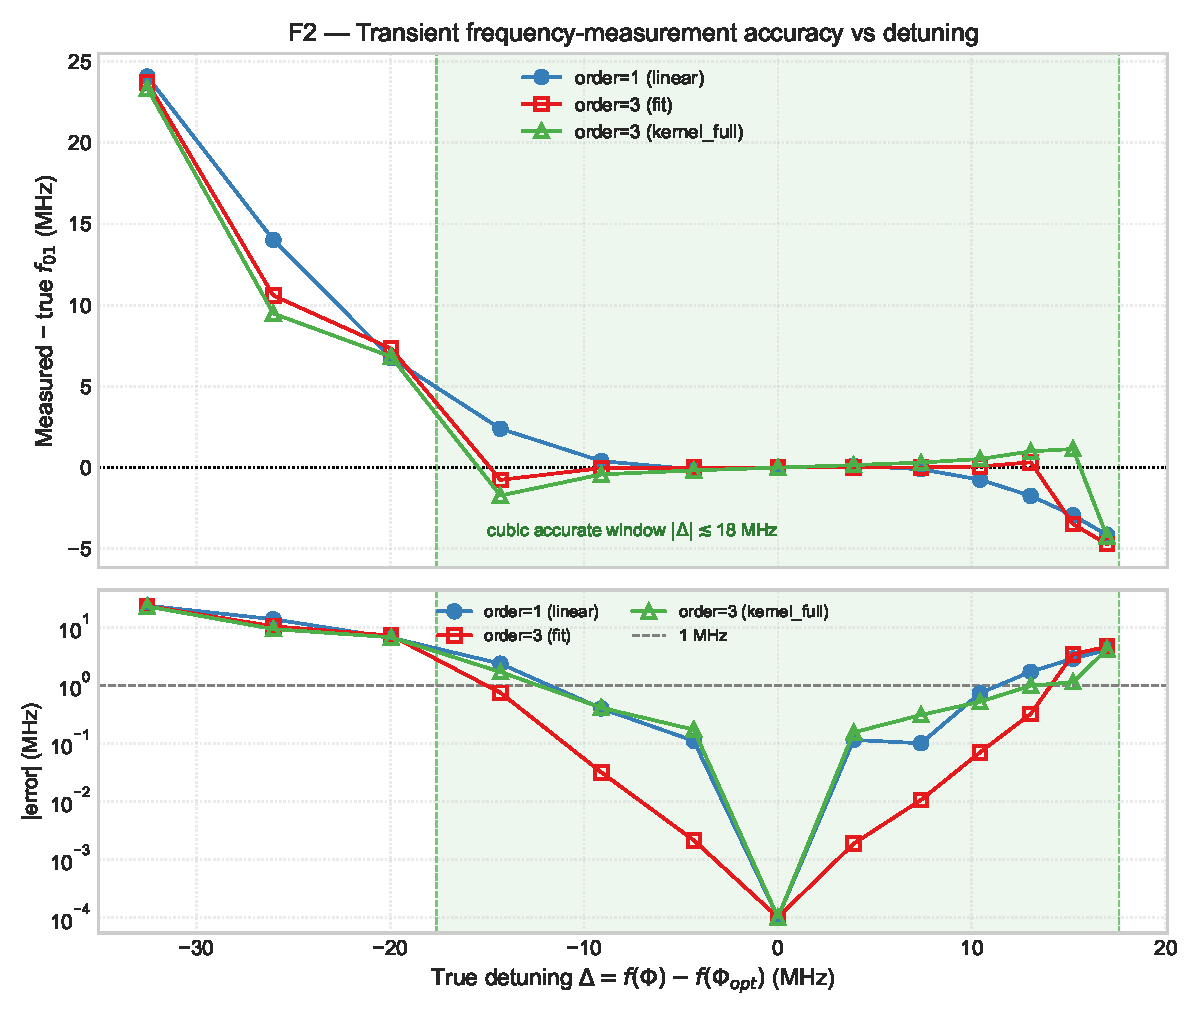
\includegraphics[width=\textwidth]{transient_accuracy.pdf}
 \caption{Accuracy of the transient frequency discriminator as a function of
 true detuning.  The upper panel shows signed measurement error and the lower
 panel its magnitude.  The shaded interval marks the cubic branch bounded by
 the response turnover.  The fixed-drive polynomial fit and full three-time
 kernel give consistent cubic corrections in the central region.}
 \label{fig:local-accuracy}
\end{figure*}

\subsection{Accuracy--cost tradeoff}

To separate estimator cost from fold failure, we next restrict the flux offsets
to $\pm0.01\Phi_0$, corresponding to $|\Delta|\lesssim12$~MHz.  Figure
~\ref{fig:pareto} compares six strategies.  Double-sweep Ramsey reaches a
6.3-kHz mean absolute error using 800 master-equation solves per frequency
measurement.  Single-sweep Ramsey configurations use 100--400 solves and give
23--30-kHz errors.  The cubic transient estimator gives a 13.5-kHz error at an
amortized cost of 18 solves per point.  Its marginal cost is two solves after a
one-time 80-solve coefficient calibration.  In this fixed-drive benchmark, the
cubic transient point Pareto-dominates all three single-sweep Ramsey settings;
double-sweep Ramsey remains more accurate at substantially higher cost.

\begin{figure*}[t!]
 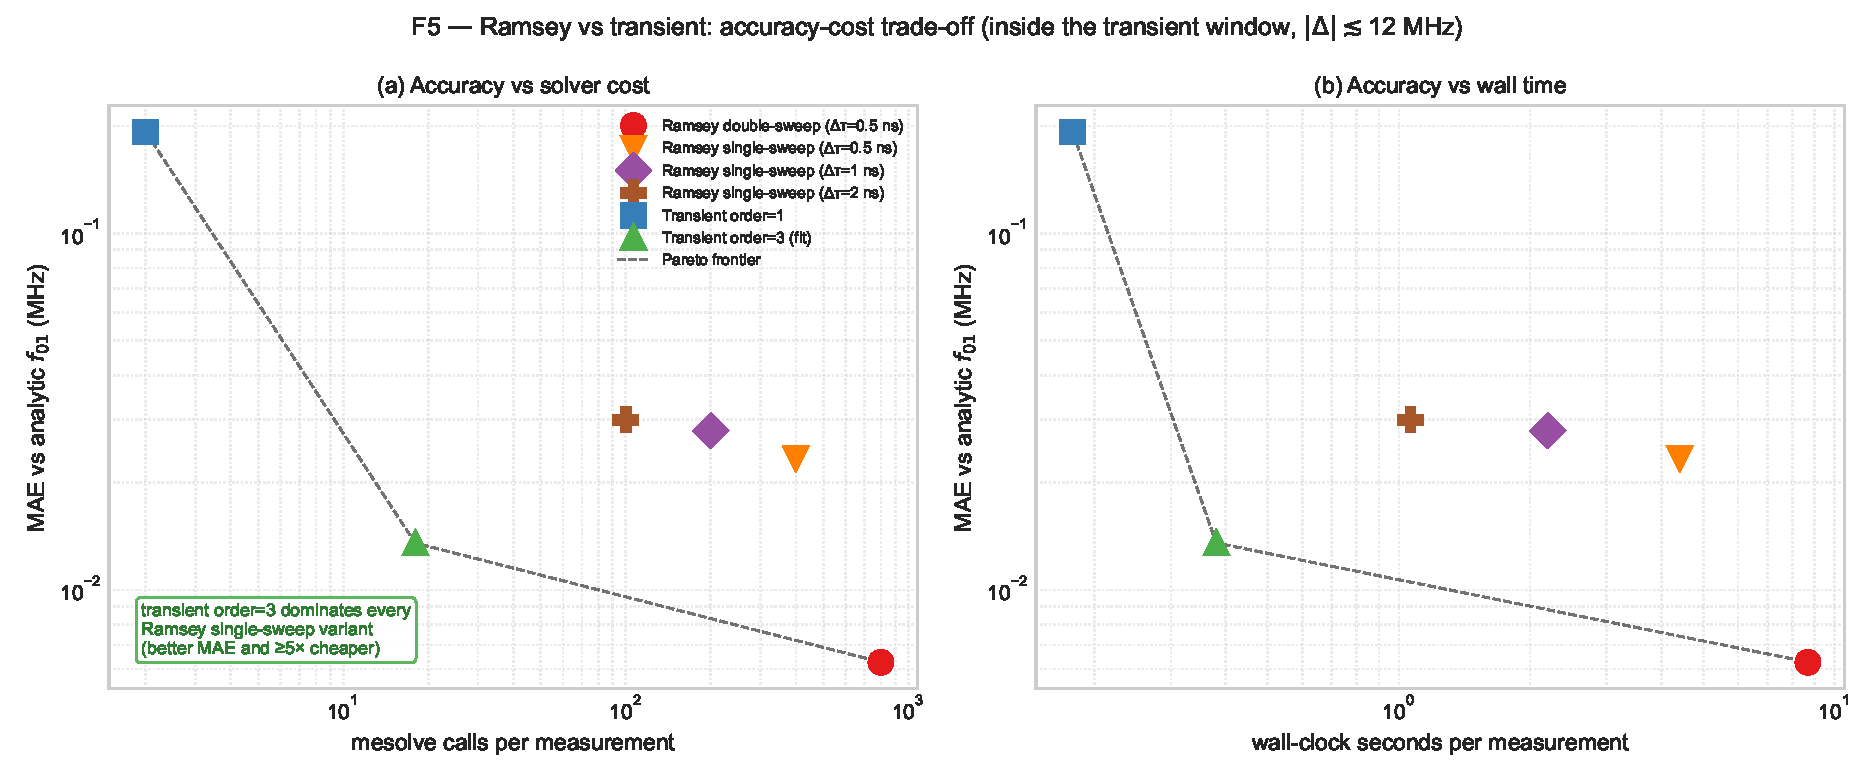
\includegraphics[width=\textwidth]{accuracy_cost.pdf}
 \caption{Accuracy--cost comparison inside the local transient window.
 (a) Mean absolute frequency error versus measured master-equation calls.
 (b) Error versus wall-clock time on the benchmark machine.  Dashed lines mark
 the nondominated frontier.  Transient cubic cost includes amortization of its
 one-time coefficient calibration over five flux points.}
 \label{fig:pareto}
\end{figure*}

\subsection{Closed-loop calibration}

We set the target frequency 20~MHz below the reference point and use the same
initial flux offset for all strategies.  Figure~\ref{fig:convergence} contrasts
three feedback loops.  A conventional double-sweep Ramsey loop converges in
five iterations.  A coarse transient stage followed by Ramsey refinement takes
seven and five iterations, respectively; the transient stage begins outside
its fold window and wanders before the handoff.  The drive-tracked transient
loop instead converges monotonically in six iterations without a Ramsey
refinement stage.

\begin{figure*}[t!]
 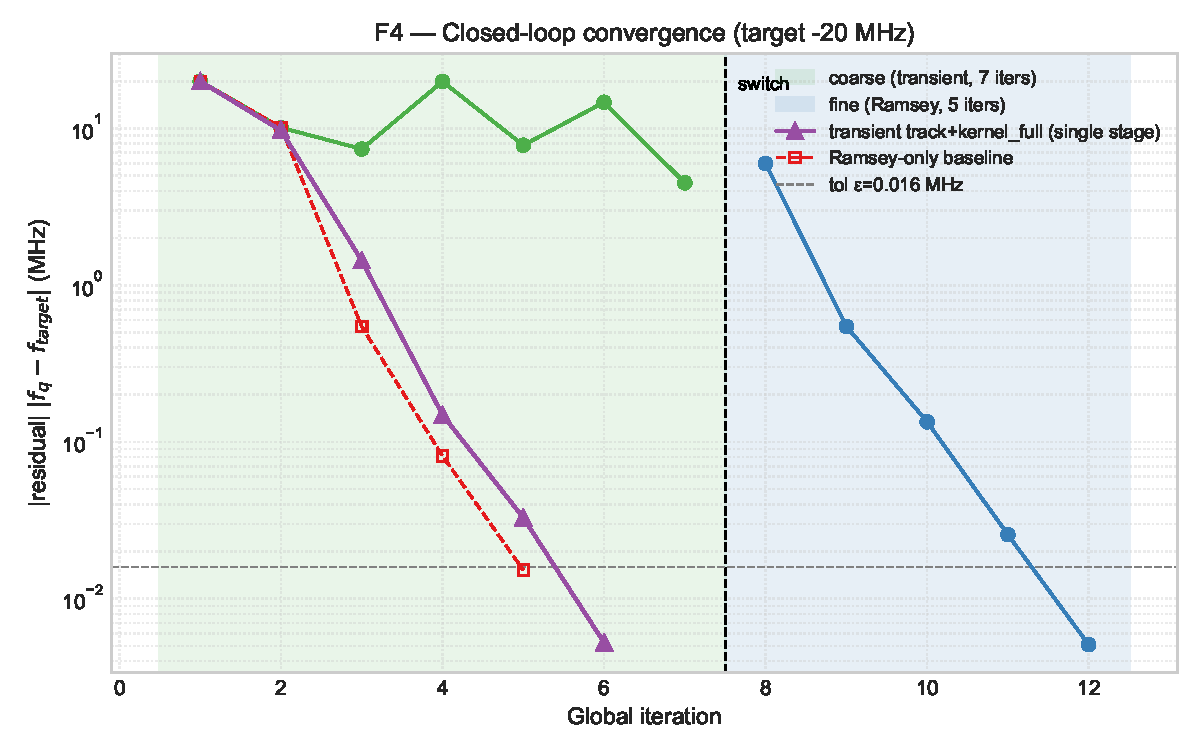
\includegraphics[width=\textwidth]{closed_loop_convergence.pdf}
 \caption{Closed-loop residual for a target shift of $-20$~MHz.  The
 coarse-to-fine workflow (green and blue regions) is compared with the
 drive-tracked full-kernel protocol (purple triangles) and a Ramsey-only
 baseline (red squares).  Residuals are independently evaluated from the
 analytic frequency--flux relation.}
 \label{fig:convergence}
\end{figure*}

Raw iteration count is not a fair cost metric because one Ramsey measurement
contains a delay scan.  We therefore instrument calls to both the master- and
Schrodinger-equation solvers and count each call with unit weight.  This is
conservative for the transient method because the state-vector solver used for
kernel evaluation is cheaper than the master-equation solver.  As shown in
Fig.~\ref{fig:closed-loop-cost}, the drive-tracked loop uses 984 counted calls
and reaches a verified residual of 0.00519~MHz.  Ramsey alone uses 4000 calls
and reaches 0.01797~MHz, giving a 4.1-fold reduction in counted cost.  The
coarse-to-fine workflow uses 5214 calls despite its 0.00214-MHz final residual;
at the common 0.016-MHz tolerance its speedup relative to Ramsey is only 0.8,
so it is more expensive rather than faster.

\begin{figure*}[t!]
 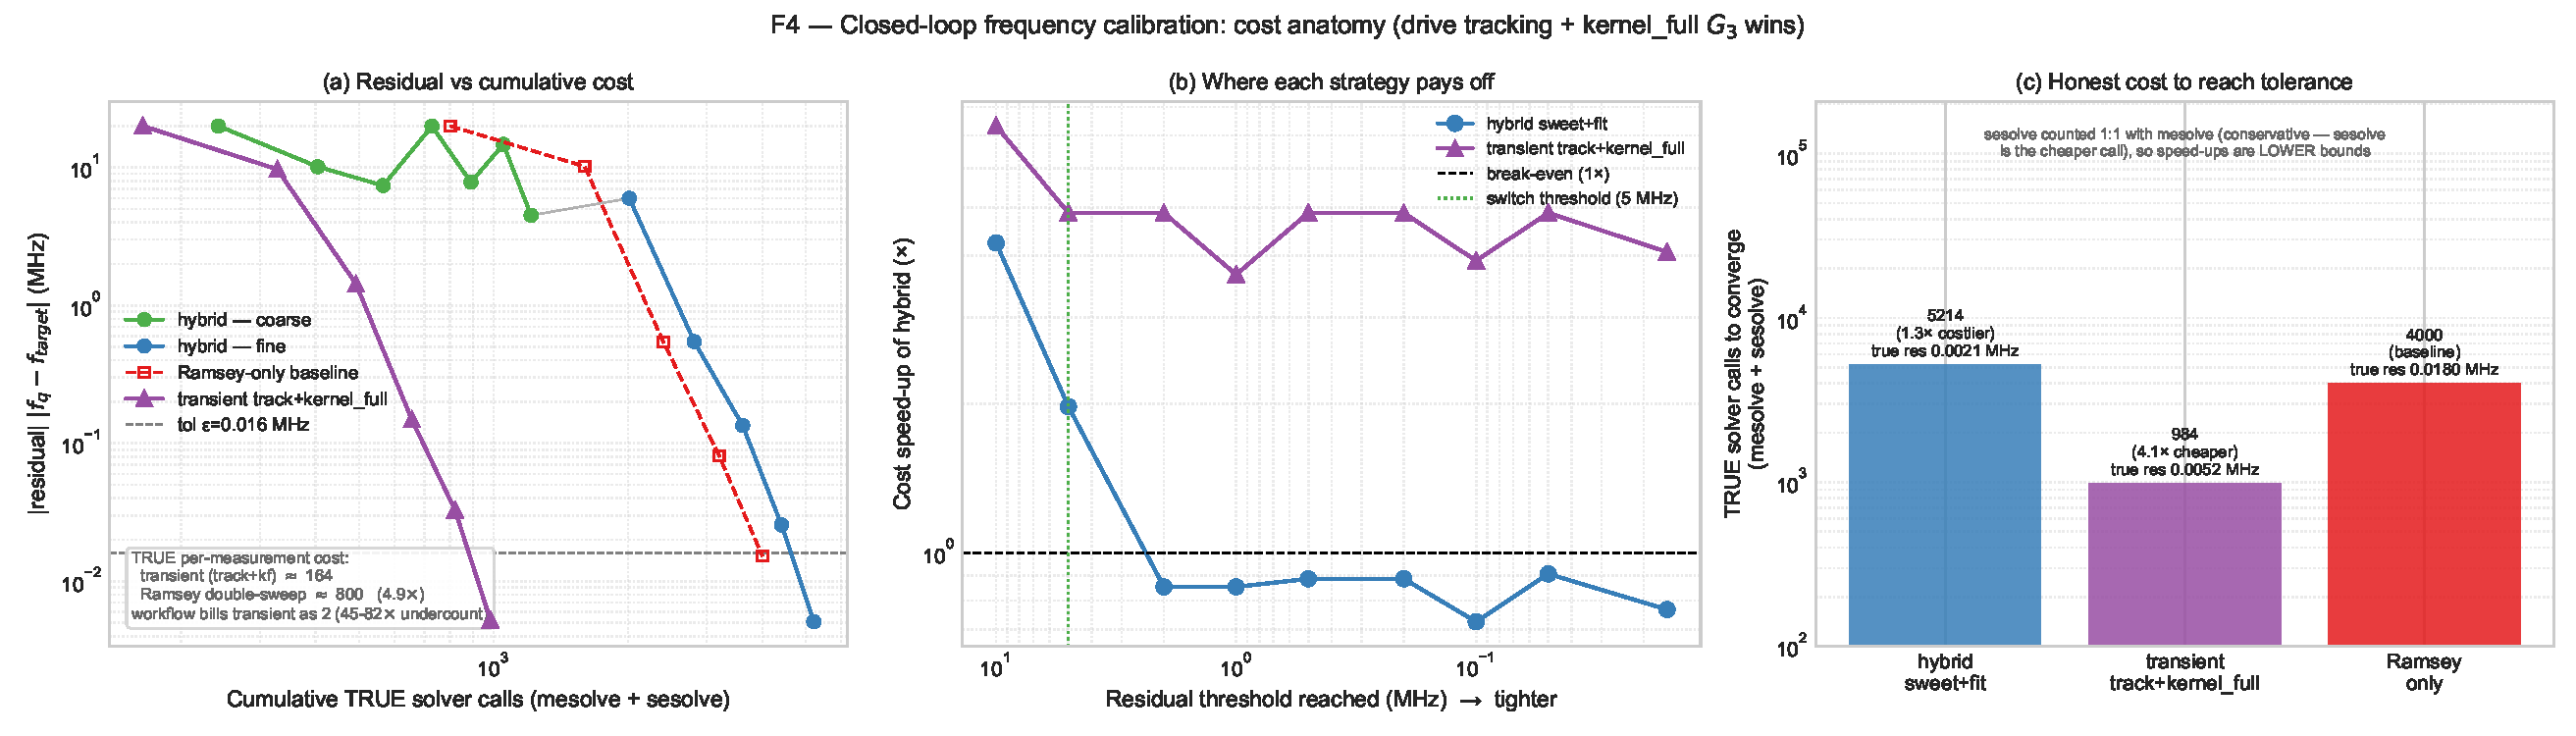
\includegraphics[width=\textwidth]{closed_loop_cost.pdf}
 \caption{Cost anatomy of closed-loop frequency calibration.  (a) Verified
 residual versus cumulative instrumented solver calls.  (b) Cost ratio relative
 to the Ramsey baseline at a common residual threshold.  (c) Total counted
 calls and independently verified final residuals.  The full-kernel transient
 route uses drive tracking; the hybrid route uses a fixed reference in its
 transient stage.}
 \label{fig:closed-loop-cost}
\end{figure*}

The mechanism is visible directly in the measured detuning.  After bootstrap,
drive tracking predicts the next transition frequency closely enough that the
probe detuning falls from sub-megahertz values to a few kilohertz while the
absolute target residual spans tens of megahertz.  The inexpensive probe thus
remains local even though the calibration travels over a nonlocal frequency
interval.  By contrast, keeping the drive fixed forces the probe itself to
span the full target displacement and crosses the turnover identified in
Fig.~\ref{fig:local-accuracy}.

\section{Discussion}
\label{sec:discussion}

% The numerical results answer the motivating question conditionally: short
% pulse sequences can contribute directly to frequency calibration, but they do
% not automatically become general-purpose frequency estimators.  The present
% two-branch sequence is a local probe, not a wide-range replacement for Ramsey
% spectroscopy.  Its cubic response reduces local nonlinear bias but cannot
% remove a response fold.  In closed loop, the useful range is preserved by
% changing the measurement reference so that the short-pulse probe stays local;
% merely assigning it to a coarse stage before an expensive fine estimator does
% not guarantee a lower total cost.

% This framing clarifies what it means for a pulse sequence to participate in
% calibration.  The sequence must encode the parameter in an observable response,
% that response must admit a calibrated inverse over a stated operating window,
% and the surrounding protocol must keep subsequent measurements inside that
% window.  In the present example, the qubit experiences constant detuning
% throughout two finite pulses, so the third-order coefficient contains
% unequal-time contributions.  A time-diagonal kernel is not the relevant
% object.  An odd-polynomial scan can recover the same coefficient when centered
% at the symmetry point, but that assumption is fragile under a moving drive.
% Evaluating the full response kernel at the actual reference frequency makes
% the short-pulse estimator and controller definitions consistent.

% The cost comparison is intentionally based on instrumented solver calls rather
% than a nominal workflow price.  The nominal price counts the two population
% measurements but can omit the solver work required to recalibrate a response
% coefficient when the drive changes.  Counting every solver invocation avoids a
% large artificial speedup.  Wall-clock time supports the same ordering in the
% present implementation, but it depends on hardware, caching, and solver choice
% and is not a universal physical metric.

% Several steps are needed before interpreting the protocol as an experimental
% calibration advantage.  The current simulations use ideal control envelopes,
% projective readout, a Markovian two-level model, and deterministic expectation
% values. Their reported uncertainty is therefore zero by construction, not a
% measured confidence interval. Shot noise, assignment error, drift during acquisition, pulse
% distortion, leakage, and imperfect knowledge of the kernel will perturb both
% the detuning estimate and the secant slope.  An experiment should report the
% number of circuit repetitions and elapsed acquisition time, and it should
% recompute the cost-to-reach curve at a common residual threshold.  A wide-range
% capture or range-guard path is also required when no reliable initial frequency
% seed is available.

% These limitations suggest a practical hierarchy rather than a replacement
% claim.  Spectroscopy or a Ramsey scan supplies acquisition and recovery.  Once
% the transition frequency is known, short-pulse sequences can participate in
% frequent local maintenance, here through a drive-tracked two-branch
% discriminator.  Occasional wide-range measurements can reinitialize the local
% loop after a range violation.  This division uses pulse-time information where
% it is unambiguous while retaining established estimators for global capture.

% The implemented state machine makes this hierarchy operational by separating
% \textsc{Verify} from \textsc{Lock}. It freezes the candidate bias during
% independent verification, sends monitor suspicion and periodic Ramsey audits
% from \textsc{Lock} through \textsc{Verify}, and reserves direct reacquisition
% for large jumps or loss of reference. These are protocol and software
% capabilities, not evidence that long-term stability has been achieved. No
% hardware time series is presently available from which to infer closed-loop
% bandwidth, frequency-noise suppression, a power spectral density, or Allan
% stability.

\section{Conclusion}
\label{sec:conclusion}

% We have investigated whether short-pulse sequences can participate directly in
% superconducting-qubit frequency calibration.  In the example studied here, a
% two-branch sequence provides a local detuning discriminator without a
% free-evolution scan.  A full third-order response kernel improves its local
% inverse, while a drive reference that tracks the predicted qubit frequency
% prevents the feedback trajectory from exhausting that local validity.  In the
% simulated 20-MHz tuning task, the protocol reduces the instrumented solver cost
% by a factor of 4.1 relative to double-sweep Ramsey and reaches a smaller
% analytically checked residual. A coarse short-pulse stage followed by Ramsey
% refinement does not provide the same advantage.

% The result demonstrates a qualified route for bringing short-pulse dynamics
% into calibration: identify a parameter-sensitive pulse response, calibrate its
% local inverse, and preserve that inverse's validity as the device moves.  It
% does not establish that short sequences replace spectroscopy or Ramsey for
% global acquisition.  Experimental validation with finite shots, readout
% error, drift, and control imperfections will determine how broadly this role
% extends and whether it reduces acquisition time on hardware.
% The extended \textsc{Acquire--Track--Verify--Lock} architecture provides a
% testable route to that validation, but the present results establish only the
% deterministic local-tracking case, not hardware verification or long-term
% locking performance.


\begin{acknowledgments}
The authors thank colleagues who contributed to discussions and experimental
support.  Funding and facility acknowledgments will be added after authorship
and grant attribution are confirmed.
\end{acknowledgments}

\appendix
\section{Numerical parameters and cost accounting}
\label{app:methods}

% The parameters used for the frozen numerical results are summarized in
% Table~\ref{tab:parameters}.  Frequencies in the simulation are angular
% frequencies; reported errors are divided by $2\pi$ and expressed in megahertz.
% Thus, for example, an angular residual $r$ in rad\,GHz is reported as
% $10^3 r/(2\pi)$ in MHz. The 0.016-MHz tolerance in Table~\ref{tab:parameters}
% is the common comparison threshold used for the frozen cost benchmark; it is
% not the independent-verification threshold of the extended state machine.

% \begin{center}
%  \refstepcounter{table}
%  \label{tab:parameters}
%  \begin{minipage}{\columnwidth}
%  \small\textsc{Table \thetable.} Parameters of the numerical calibration
%  benchmark.\par\smallskip
%  \centering
%  \begin{tabular}{lc}
%  \toprule
%  Parameter & Value \\
%  \midrule
%  $E_C/h$ & $0.2$ GHz \\
%  $E_J/h$ & $10$ GHz \\
%  Reference flux & $0.9553166\Phi_0$ \\
%  $T_1$ & $100~\mu$s \\
%  $T_2$ & $50~\mu$s \\
%  Hilbert-space dimension & 2 \\
%  Sampling interval & $0.5$ ns \\
%  $\pi/2$ pulse window & $10$ ns \\
%  Closed-loop target shift & $-20$ MHz \\
%  Residual tolerance & $0.016$ MHz \\
%  Damping factor & $0.8$ \\
%  Maximum flux step & $0.02\Phi_0$ \\
%  \bottomrule
%  \end{tabular}
%  \end{minipage}
% \end{center}

% For the accuracy--cost benchmark, Ramsey free-evolution times span
% $0\leq\tau<200$~ns with spacings of 0.5, 1, or 2~ns.  Double-sweep Ramsey uses
% two artificial-detuning scans; single-sweep Ramsey uses one.  The transient
% measurement requires two final-state simulations.  The fitted cubic route pays
% an additional one-time calibration cost, which is amortized across the five
% flux offsets in Fig.~\ref{fig:pareto}.

% The closed-loop benchmark instruments all calls made through the frequency
% measurement and kernel-estimation paths.  Calls to the master-equation solver
% and the state-vector solver are assigned equal unit cost.  The latter is
% typically cheaper, so the reported transient advantage in solver-call units is
% conservative.  Final residuals are recomputed from the analytic transmon
% dispersion at the returned flux point and are not taken from the internal
% measurement history.

% \subsection{State-machine thresholds and data separation}

% The extended protocol uses the angular-frequency hierarchy
% Eq.~\eqref{eq:threshold-hierarchy}. The reference runtime configuration is
% $\epsilon_{\mathrm{hold}}/(2\pi)=0.010$~MHz,
% $\epsilon_{\mathrm{final}}/(2\pi)=0.100$~MHz,
% $\epsilon_{\mathrm{enter}}/(2\pi)=5$~MHz, and
% $\Delta_{\mathrm{val}}/(2\pi)=20$~MHz. These values define software policy
% for the state-machine implementation; they were not used to generate a
% finite-shot or long-term hardware data set in this work.

% For statistical measurements, the uncertainty allowance in
% Eq.~\eqref{eq:track-verify-statistics} is $z_{1-\beta}\sigma$, where the coverage
% level $1-\beta$, the estimator for $\sigma$, and any multiple-testing policy
% must be fixed before data acquisition. The deterministic QuTiP executor used
% for the present numerical examples returns exact expectation values and sets
% $\sigma=0$ with the explicit provenance tag
% \texttt{uncertainty\_source=deterministic\_zero}. This zero must not be
% interpreted as an experimentally measured confidence interval.
% The runtime represents $z_{1-\beta}$ explicitly as a configured confidence
% multiplier. A \textsc{Track} event carries probe detuning and probe-detuning
% uncertainty separately from the target residual; a missing or invalid probe
% quantity rejects the local estimate rather than substituting the residual.

% The reference verification policy requires $N_{\mathrm{verify}}=2$
% consecutive passes at a frozen candidate bias, permits at most five attempts
% and $10^4$ verification shots per episode, and enforces a bias-freeze
% tolerance of $10^{-12}\Phi_0$. A failed but locally valid measurement returns
% to \textsc{Track}; an ambiguous or locally invalid measurement enters
% \textsc{Reacquire}. Command, shot, solver-call, wall-time, retry, and
% reacquisition budgets are checked before a measurement command is executed.
% Exhaustion, cancellation, or an interlock enters \textsc{SafeStop} and applies
% a safe hold.

% Let $T_{\mathrm{mon}}$ denote the interval between low-cost \textsc{Lock}
% checks and $T_{\mathrm{audit}}$ the interval between independent Ramsey
% audits. A monitor statistic below the calibrated clear threshold retains
% \textsc{Lock}; three consecutive readings in the suspect band, or an elapsed
% $T_{\mathrm{audit}}$, enter \textsc{Verify}. A large jump enters
% \textsc{Reacquire}. In the current deterministic runtime defaults,
% $T_{\mathrm{mon}}=0$ requests a check on every loop and
% $T_{\mathrm{audit}}=0$ disables periodic audits. Positive intervals must be
% chosen and frozen for a long-running hardware experiment; no such time series
% is reported here.
% The compatibility default therefore leaves periodic auditing optional, while
% the long-running configuration can require a positive audit interval. Monitor
% retention and satisfaction of $\epsilon_{\mathrm{hold}}$ are recorded as
% separate outcomes; the former does not by itself establish the latter.

% Four data roles are kept separate. Response-calibration data determine
% $G_1$, $G_3$, and nuisance corrections. Held-out response-validation data
% determine $\Delta_{\mathrm{val}}$ and test the local inverse. Closed-loop
% independent-verification data evaluate Eq.~\eqref{eq:verification-condition}
% at the frozen candidate bias. Long-term monitoring data evaluate drift after
% entry to \textsc{Lock}. The analytic frequency--flux calculation used to
% score the deterministic benchmark is simulation ground truth and is not
% substituted for either of the latter two experimental data roles.

% The runtime checkpoints the complete state, budgets, tracker state, frozen
% candidate, and pending command. Recovery has at-least-once execution
% semantics: a pending command retains its original command identifier, so the
% executor must be idempotent with respect to that identifier. Cancellation and
% keyboard interruption request a checkpoint before the safe-hold transition.


\bibliography{references}

\end{document}
